%!TEX root=main.tex
\section{Parallelizing in FPGA}
\label{sec:optimization}

As discussed in \S\ref{subsec:fpga}, it is critical to fully utilize the parallelism inside FPGA in order to speed up processing.
\name\ exploits FPGA parallelism both at element-level and inside an element.

\subsection{Parallelism across elements}

The modular architecture of \name\ makes it natural to exploit parallelisms across different elements.
The \name\ tool-chain maps each element into a hardware block in FPGA. 
These logic blocks are interconnected with FIFO buffers, and can work completely in parallel.
%
To this end, one can think of each element in a \name\ configuration as a tiny, independent core with customized logic.
Packets flow from one element to another along a \textit{processing pipeline}.
This type of parallelism is called \textit{pipeline parallelism} or \textit{task parallelism}. % (Figure~\ref{fig:element-para}(a)).
%
Furthermore, if a single processing pipeline does not have enough processing power, we can duplicate multiple such pipelines 
in FPGA and divide data into these pipelines using a load-balancing element, \ie, exploiting \textit{data parallelism}. %(Figure~\ref{fig:element-para}(b)).
For network traffic, there are both data parallelism (at packet-level or flow-level)
and pipeline parallelism that can be utilized  to speed up processing.
\name\ is very flexible and can be configured to capture both types of parallelism with little efforts.

\egg{
\begin{figure}
\centering
\begin{tabular}{c}
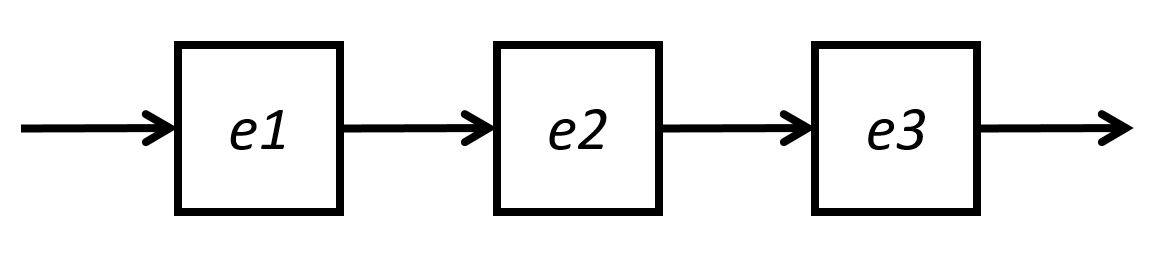
\includegraphics[width=0.28\textwidth]{pipeline.jpg}\\
(a)\\
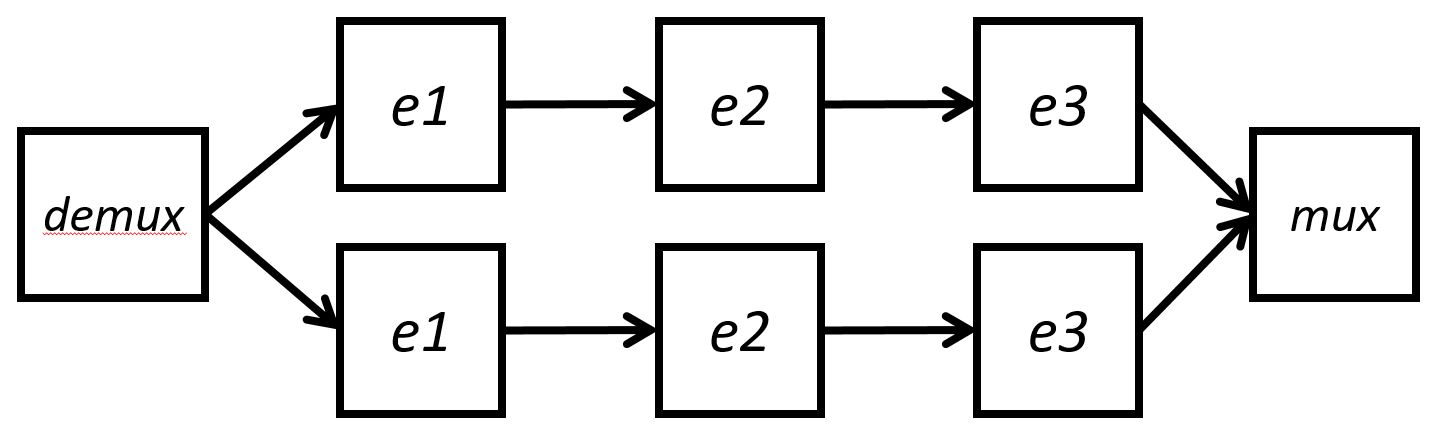
\includegraphics[width=0.35\textwidth]{data.jpg}\\
(b)\\
\end{tabular}
\caption{(a) Pipeline parallelism among elements. (c) Data parallelism among elements.}
\label{fig:element-para}
\end{figure}
}

\subsection{Parallelism inside element}
\label{subsec:paral_in_elem}

%
% We need to get the processing pipeline concept clear here.
%
Unlike CPU, which executes instructions in memory with limited parallelism, 
FPGA synthesizes operations into hardware logic, and therefore
can be evaluated in parallel without instruction load overhead.
If a datum requires multiple dependent
operations in one handler function, HLS tools will 
schedule these operations into pipeline stages in a synchronized manner. 
At every clock, the result of one stage moves to the next stage, and 
at the same time, a new datum is inputed into this stage, as shown in
Figure~\ref{fig:dependency}(a).
This way, the handler function can process a datum at every clock cycle
and achieve maximum throughput.
%
However, in practice, this efficient pipeline processing 
could break under two situations: (1) there is \textit{memory dependency} among operations; 
and (2) there are \textit{unbalanced} stages.
%
In the following two subsections, we will discuss these two issues in 
details and present our solutions.
%Finally, in \S~\ref{subsubsec:pipeline-control}, we discuss how to explicitly
%control the pipelining to get better clock frequency in \name.



\subsubsection{Minimize memory dependency}

\begin{figure}
\lstset{style=numbers}

\lstset{ emph={%
 element, init, state, handler, signal,include
}, emphstyle={\bfseries .},
morekeywords={get_input_port,read_input_port,from_tor, to_tor, set_output_port, host} 
}

\centering
\begin{tabular}{c}

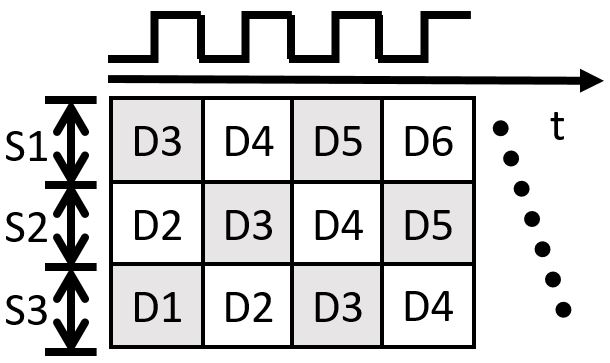
\includegraphics[width=.25\textwidth]{pipeline-w-data.jpg} \\
(a) \vspace{3pt} \\
{
\scriptsize 
\begin{lstlisting}[escapechar=@]
    r = read_input_port (PORT_1);
S1: y = mem[r.x]+1;
S2: mem[r.x] = y;
    set_output_port (PORT_1, y);
\end{lstlisting} 
}\\
(b) \vspace{3pt}\\
{
\scriptsize 
\begin{lstlisting}[escapechar=@]
    r = read_input_port (PORT_1);
P1: if ( r.x == buf_addr ) {
       y_temp = buf_val;
    } else {
       y_temp = mem[r.x];
    }
    mem[buf_addr] = buf_val;   
S1: y = y_temp + 1;
S2: buf_addr = r.x;
    buf_val  = y;
    set_output_port (PORT_1, y);
\end{lstlisting} 
}\\
(c)
\end{tabular}
\caption{Illustration of dependency. (a) No dependency. S$n$ means a pipeline stage, D$n$ is a datum. (b) Memory dependency occurs when states are stored in memory and need to be updated. (c) Resolve memory dependency using delayed write.}
\vspace{-10pt}
\label{fig:dependency}
\end{figure}

% registers
\egg{
\smalltitle{Use registers.}
Unlike CPU, which executes instructions in memory one by one, FPGA synthesizes 
operations into hardware logic and stores data in registers, and therefore 
can be evaluated in parallel.
For example, Figure~\ref{fig:dependency}(a), it may take a CPU two cycles 
to execute \textbf{S1} and \textbf{S2}, while in FPGA, the value of variable 
\textit{y} and \textit{z} can be evaluated in one cycle using 
combinational logic, if we store all variables in registers.
FPGA usually has a large number of registers, \ie, 697Kbit for Altera 
Stratix V, and therefore \name\ aggressively assigns scalar variables 
using registers to increase the parallelism.
}

%\smalltitle{Minimize memory dependency.}
If two operations access the same memory location, and at least one of them
is \textit{write}, we call these two operations depend on each other~\cite{dependence}. 
Operations with \textit{memory dependency} cannot be evaluated at the same time,
as each memory access has one cycle latency and the semantic correctness of the program strongly depends on the order
of operations.
%
As shown in Figure~\ref{fig:dependency}(b), \textbf{S1} and \textbf{S2}
depend on each other: \textbf{S2} has to be delayed until \textbf{S1} finishes, 
and only after \textbf{S2} finishes can \textbf{S1} operate on new input data.
Therefore, the function will take two cycles to process one datum.
%
Memory dependency can be rather complicated for some processing algorithms,
but thanks to the modular architecture of \name, most elements perform 
only simple tasks and the \textit{read-write} memory dependency shown in 
Figure~\ref{fig:dependency}(b) is the most common case we have encountered.

One way to remove this memory dependency is to store data in registers only. 
%
Since registers are fast enough to perform read, computation and write back within one cycle,
there would be no \textit{read-write} dependency at all. 
Indeed, compared to CPU, FPGA has a much larger number of 
registers, \ie, 697Kbit for Altera Stratix V, which can be used
whenever possible to reduce memory dependency.
The \name\ compiler aggressively assigns registers to variables as long as
all accesses to the variable refer to a constant address -- either the variable is a scalar or an array entry with constant offset.
%
Certainly, the programmer can use ``register'' or ``local/global'' keywords to explictly instruct the compiler to place a variable (can also be an array)
in register, BRAM or onboard DDR memory.
%declare the  in array declaration to force the compiler to use registers and generate multiplexers for memory access.}

For large data, they have to be stored in memory. 
%
Fortunately, we can still use a technique called \textit{delayed write} to
resolve the \textit{read-write} memory dependency in Figure~\ref{fig:dependency}(b).
The core idea is to buffer the new data in a register and delay the write
operation until the next read operation. 
If the next read accesses the same location, it will read the value from
the buffer register directly. Otherwise, the read can operate in parallel 
with the delayed write operation as they are going to access different
memory locations\footnote{Most BRAM in FPGA has two ports.}.
Figure~\ref{fig:dependency}(c) shows the code snippet with delayed write.
Since there is no longer memory dependency in the code, the element can 
process a datum in one cycle.
%
By default, \name\ compiler automatically applies \textit{delayed write} 
for an array (generating similar code as shown in Figure~\ref{fig:dependency}(b)).
%
\egg{But Currently the compiler can generate only one delayed write per array.
For complex memory dependencies, the programmer should rewrite the code into multiple elements accessing disjoint memory regions, and use message-based coordination if necessary.}


\begin{figure}
\lstset{style=numbers}

\lstset{ emph={%
 element, init, state, handler, signal,include,state\_machine, goto_state
}, emphstyle={\bfseries},
morekeywords={get_input_port,read_input_port,from_tor, to_tor, set_output_port, host, begin, VLAN, IPv4, GRE} 
}
\centering


\begin{tabular}{cc}
\scriptsize 
\begin{lstlisting}[escapechar=@]
struct hash_entry
{
  ulong key;
  ulong cnt;
} A[100];

.handler {
  ...
  idx = hash (h);
S1: if (A[idx].key==k)
  {
S2: A[idx].cnt ++;
  }
  ...
}
\end{lstlisting} &
\raisebox{-60pt}{
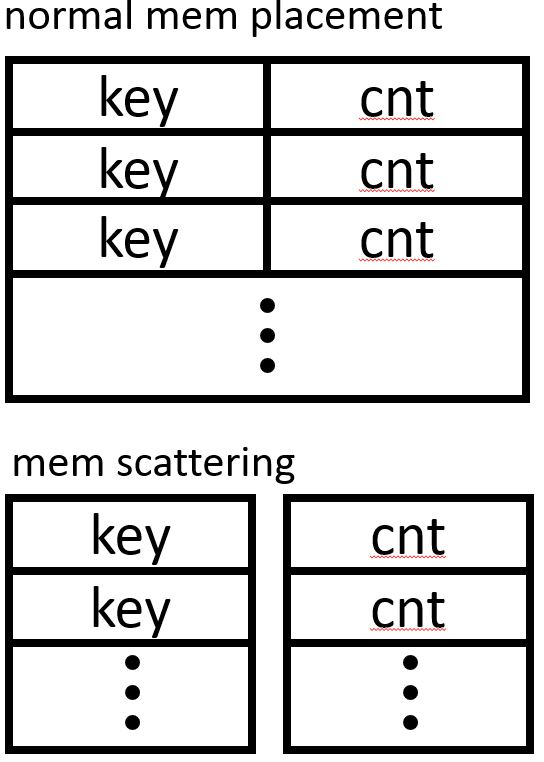
\includegraphics[width=.17\textwidth]{mix.jpg} }\\
(a) & (b)
\end{tabular}
\vspace{-10pt}
\caption{Memory scattering. }
\vspace{-15pt}
\label{fig:memscattering}
\end{figure}


%\smalltitle{Remove pseudo-dependency.}
One subtle issue will occur when using an array of \textit{struct} variables. 
Figure~\ref{fig:memscattering}(a) shows such an example, where
a hash table is used to maintain a count for every flow.
We find \textbf{S2} will have a memory dependency to \textbf{S1}, although
they are accessing different fields of a \textbf{struct}.
The reason is that almost all current HLS tools will treat a \textbf{struct}
array as a single-dimension array with a large bit-width -- equal to
the size of the \textbf{struct}, and use only one arbitrator to control 
 access.
We call this type of memory dependency \textit{pseudo dependency}, 
as physically, the two fields, \textit{key} and \textit{cnt}, can be on different 
memory locations.
%
To resolve this issue, \name\ employs a simple technique called \textit{memory scattering}, which automatically 
translates a \textbf{struct} array into several 
independent arrays, each for a field in the \textbf{struct}, and assigns them into different BRAMs (Figure~\ref{fig:memscattering}(b)).
With \textit{memory scattering}, \textbf{S1} no longer depends on \textbf{S2}.
So the pipeline can be inferred by HLS tools, and when \textbf{S2} is 
still operating, a new datum can be clocked in and processed 
by \textbf{S1}.
It is worth noting that memory scattering is only applied for elements 
in FPGA and disabled if elements are assigned to run on the host CPU.

We note that the above techniques may not resolve all memory dependencies. 
In many cases, it requires programmers to re-factor their code or even change
the algorithms to ensure their implementation can be fully pipelined in FPGA. 

\egg{
\begin{figure}
\lstset{style=numbers}

\lstset{ emph={%
 element, init, state, handler, signal,include,state\_machine, goto_state
}, emphstyle={\bfseries},
morekeywords={get_input_port,read_input_port,from_tor, to_tor, set_port_output, host, begin, VLAN, IPv4, GRE} 
}
\centering

\begin{tabular}{c|c}
% left
\begin{tabular}[t]{c}
\scriptsize 
\begin{lstlisting}[escapechar=@]
struct hash_entry
{
    ulong key;
    ulong val;
} A[100];

.handler {
   ...
   idx = hash (h);
   @\textbf{k = A[idx].key;}@
   @\textbf{v = A[idx].val;}@
   if (h == k) 
      ret = v;
   ...
}
\end{lstlisting} \\
\normalsize (a) \vspace{10pt} \\
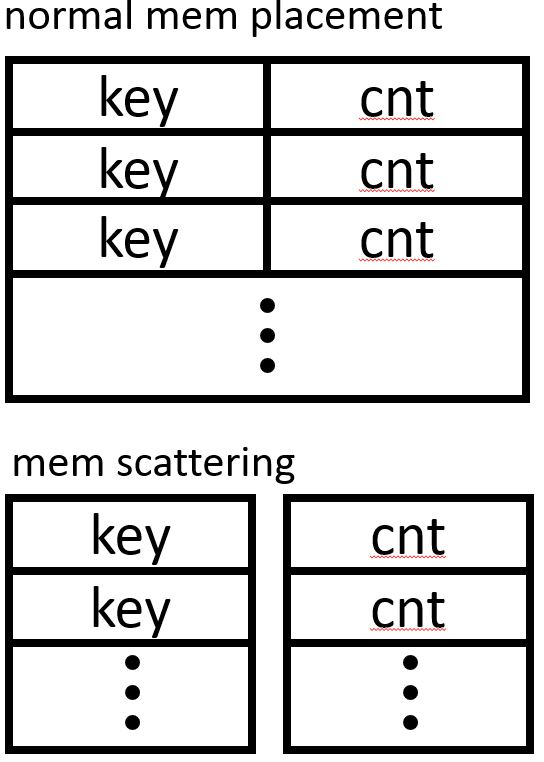
\includegraphics[width=.2\textwidth]{mix.jpg} \\
\normalsize (b) \vspace{10pt} \\
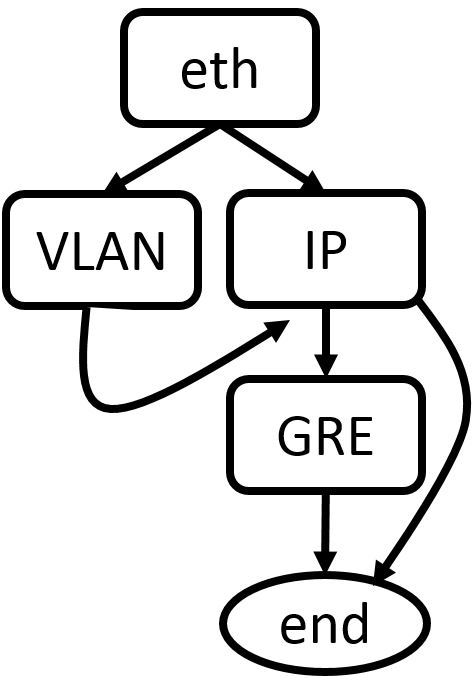
\includegraphics[width=.15\textwidth]{fsm1.jpg} \\
\normalsize (d) \\
\end{tabular}
&
\raisebox{-150pt}{
\begin{tabular}{c}
\begin{lstlisting}[escapechar=@]
.handler {
 ...
 .state_machine
 {
  begin { // ethernet
   ...
   if(etype==0x8100)
    .goto_state VLAN;
   else 
   if(etype==0x0800)
    .goto_state IPv4;
   else
    .goto_state end;
  }
  VLAN {
    ...
    if(etype==0x0800)
     .goto_state IPv4;
    else
     .goto_state end;
  }
  IPv4 {
    ...
    if(proto==0x2F)
     .goto_state GRE;
    else
     .goto_state end;
  }
  GRE {
   .goto_state end;
  }
 }  
...
}

\end{lstlisting}  \\
\normalsize (c) \vspace{10pt} \\
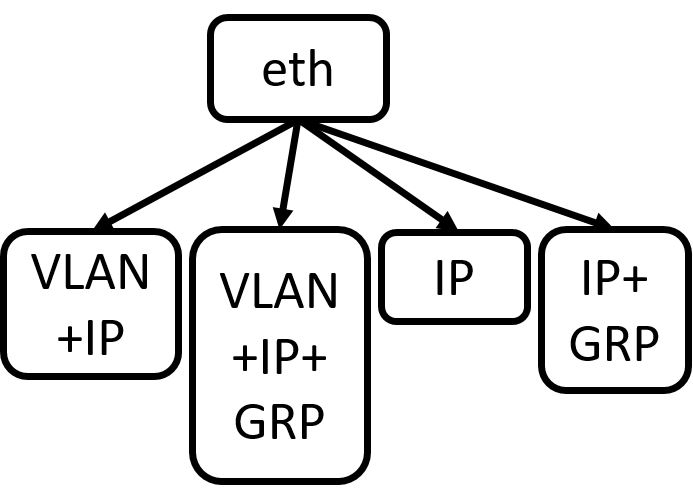
\includegraphics[width=.2\textwidth]{fsm2.jpg} \\
\normalsize (e) \\
\end{tabular}
}

\end{tabular}

\caption{Memory scattering (a, b) and FSM expansion (c-e). }
\label{fig:memscattering}
\end{figure}
}

\subsubsection{Balance pipeline stages}
Ideally, we require every stage in one processing pipeline to have the same speed. \ie, processing a datum at one clock cycle.
However, if the process at each stage is unbalanced and some stages need more cycles than others, these fat stages will
limit the whole throughput of the pipeline.  
For example, in Figure~\ref{fig:unbalance}(a), \textbf{S1} is a loop operation. 
Since each iteration takes one cycle (\textbf{S2}), the whole loop will need $N$ cycles to finish, significantly reducing the pipeline
throughput.
Figure~\ref{fig:unbalance}(b) shows another example, which implements a cache in BRAM for a global table (\textit{gmem}) in DDR.
Although the ``else'' branch is seldom hit, it generates a fat stage in the 
pipeline (taking hundreds of cycles!), and slows down
the processing greatly.

\name\ uses two techniques to balance the stages inside a pipeline. First, we \textit{unroll} the loop whenever possible. 
When unrolled, the loop operation effectively breaks into a sequence of small operations, each of which can be finished in one cycle.
It is worth noting that unrolling a loop will duplicate the operations in the loop body and thus increase area cost. 
Therefore, it may be only applicable to loops with simple bodies and 
small number of iterations. 
In NFs, we find such small loops are rather common, \eg calculating checksums, shifting packet payload and iterating through possible configurations.
ClickNP compiler provides the \textbf{.unroll} directive to unroll a loop. 
%
While many HLS tools support loop unroll for a known number of iterations, 
ClickNP extends this capability to unroll a loop whose  
number of iterations is unknown but under an upper bound 
that is specified by programmers.

Second, if we identify that an element has both heavy and light-weight operations, we try to separate each type of operations in an individual element.
For example, to implement a cache as shown in Figure~\ref{fig:unbalance}(b), we move the slow ``else'' branch into another element.
This way, the fast path and the slow path would be running asynchronously.
If cache miss is rare, the overall processing speed is dominated by the fast path.
We will return to this point later in \S\ref{sec:application}.
Currently, \name\ compiler cannot automatically perform such separation for 
programmers.

\begin{figure}
\lstset{style=numbers}

\lstset{ emph={%
 element, init, state, handler, signal,include,state\_machine, goto_state
}, emphstyle={\bfseries},
morekeywords={get_input_port,read_input_port,from_tor, to_tor, set_output_port, host, begin, VLAN, IPv4, GRE} 
}
\centering

\begin{tabular}{c}
{
\scriptsize 
\begin{lstlisting}[escapechar=@]
.handler {
   r = read_input_port (PORT_1);
   ushort *p = (ushort*) &r.fd.data;
S1:for (i = 0; i<N; i++) {
S2:  sum += p[i];
   }
}
\end{lstlisting} 
} \\
(a) \vspace{3pt} \\
{
\scriptsize 
\begin{lstlisting}[escapechar=@]
.handler {
   r = read_input_port (PORT_1);
   idx = hash (r.x);
S1:if ( cache[idx].key == r.x ) {
     o = cache[idx].val;
S2:} else {
     o = gmem[r.x];
     k = cache[idx].key;
     gmem[k] = cache[idx].val;
     cache[idx].key = r.x;
     cache[idx].val = o;
   }
   set_output_port (PORT_1, o);
}
\end{lstlisting} 
} \\
(b) \vspace{3pt} 
\end{tabular}

\caption{Unbalanced pipeline stages. }
\label{fig:unbalance}
\vspace{-10pt}
\end{figure}


\egg{
\smalltitle{Expand code.} \name\ provides several tools to help programmers to expand code, trading off FPGA area for speed.
One common code expansion is to unroll loops. Additionally, \name\ provides \textit{.repeat} directive to expand code according to
a template.
Finally, \name\ can also help to expand a \textit{finite state machine} (FSM).
Figure~\ref{fig:memscattering}(c) shows such an example in packet header parser.
The \textbf{.state\_machine} directive has two functions. First, it provides programmers a declarative way to write a FSM by defining
states and their transitions (using \textbf{.goto\_state}).
Second, it also expends the FSM to get more parallelism. 
For example, Figure~\ref{fig:memscattering}(d) shows the parsing tree that is described according to the code piece in Figure~\ref{fig:memscattering}(c).
But \name\ compiler can automatically expends the FSM to an equivalent, but much flattened FSM, as shown in Figure~\ref{fig:memscattering}(e). Now every header can be parsed in one cycle -- all parsing paths can be evaluated in parallel, 
instead of up to 4 cycles (Figure~\ref{fig:memscattering}(d)).
}

\egg{
\subsubsection{Explict pipeline control}
\label{subsubsec:pipeline-control}

While commercial HLS tools can automatically generate pipeline structure, it is not always perfect. 
One issue that we are facing occasionally is that HLS tools may too aggressively use large block of combinational logic 
to implement operations in a handler function.
Although packing more operations in a combinational logic makes all these operations be evaluated in parallel in one clock,
it may also reduce the clock frequency of the FPGA as the frequency is restricted by the delay of the logic block, and larger
the block, longer the delay.
%
For example, Figure~\ref{fig:pipeline-control}(a) shows such an example. The code snippet selects the maximal value from
a set of registers (as we will show later, this is a foundation for priority scheduling).
Since all data are in registers, most HLS tools will aggressively use a large block of combinational logic to implement, so that
all \textbf{if} operations are evaluated in one clock cycle. However, this will cause a low frequency of xxx MHz. 
As shown in Figure~

}